% v2-acmtog-sample.tex, dated March 7 2012
% This is a sample file for ACM Transactions on Graphics
%
% Compilation using 'acmtog.cls' - version 1.2 (March 2012), Aptara Inc.
% (c) 2010 Association for Computing Machinery (ACM)
%
% Questions/Suggestions/Feedback should be addressed to => "acmtexsupport@aptaracorp.com".
% Users can also go through the FAQs available on the journal's submission webpage.
%
% Steps to compile: latex, bibtex, latex latex
%
% For tracking purposes => this is v1.2 - March 2012
\documentclass{acmtog} % V1.2

%\acmVolume{VV}
%\acmNumber{N}
%\acmYear{YYYY}
%\acmMonth{Month}
%\acmArticleNum{XXX}
%\acmdoi{10.1145/XXXXXXX.YYYYYYY}

\acmVolume{}
\acmNumber{}
\acmYear{2016}
\acmMonth{May}
\acmArticleNum{}
\acmdoi{}

\begin{document}

\markboth{V. I. Shaytan}{Developing a testing system for Functional Programming course}

\title{Developing a testing system for Functional Programming course} % title

%%\author{VITOR F. PAMPLONA {\upshape and} MANUEL M. OLIVEIRA
\author{VASILY I. SHAYTAN
\affil{Saint-Petersburg State University}
%%%\and
%%%GLADIMIR V. G. BARANOSKI
%%%\affil{University of Waterloo}
%%%\and
%%%SEAN FOGARTY
%%%\affil{University of Illinois at Urbana-Champaign}
% NOTE! Affiliations placed here should be for the institution where the
%       BULK of the research was done. If the author has gone to a new
%       institution, before publication, the (above) affiliation should NOT be changed.
%       The authors 'current' address may be given in the "Author's addresses:" block (below).
%       So for example, Mr. Fogarty, the bulk of the research was done at UIUC, and he is
%       currently affiliated with NASA.
}
%%%D.1.1 [Programming Techniques]:
%%%Applicative (Functional) Programming; D.3.2 [
%%%]: Language Classifications—Applicative (functional)
%%%languages; K.3.2 []: Computer
%%%and Information Science Education—Computer science education
\category{D.1.1}{Programming Techniques}{Applicative (Functional) Programming}
\category{D.3.2}{Programming Languages}{Language Classifications-Applicative (functional) languages}
\category{K.3.2}{Computers and Education}{Computer and Information Science Education—Computer science education}
%%%\category{I.3.5}{Computer Graphics}{Computational Geometry and Object Modeling}[Physically based modeling]

\terms{Algorithms, Languages, Reliability}

\keywords{Haskell, functional programming, testing,
monads, education}

%%%\acmformat{Vitor F. Pamplona, Manuel M. Oliveira, Gladimir V. G. Baranoski,
%%%and Sean Fogarty. 2009. Photorealistic models for pupil light reflex and iridal pattern deformation.
%%{\em ACM Trans. Graph.} 28, 4, Article 106 (September 2009), 10 pages.\\
%%\doiline}

\maketitle

%%%\begin{bottomstuff}
%%%Manuel M. Oliveira acknowledges a CNPq-Brazil fellowship (305613/2007-3). Gladimir V. G. Baranoski acknowledges a
%%%NSERC-Canada grant (238337). Microsoft Brazil provided additional support.
%%%Authors' addresses: Sean Fogarty, (Current address) NASA Ames Research Center, Moffett Field, California 94035.
%%%\end{bottomstuff}


\begin{abstract}
We report on our experience teaching a Haskell-based functional
programming course to over 400 students for four autumn terms.
The syllabus was organized around selected material from various
sources. Throughout the terms, we emphasized correctness through tests and proofs. The submission architecture
was coupled with hand and automatic testing, giving students the possibility
to correct mistakes before the deadline. To motivate the students,
we complemented the weekly assignments with an informal
competition and gave away points in a end course.
\end{abstract}

\section{Introduction}

This paper reports on a mandatory Haskell-based functional programming course at the Saint-Petersburg State University. In the
first iteration (autumn-winter semester of 2012-2013), there were 32 students
enrolled. In the following autumn-winter semester (2016-2017), there
were 80 students enrolled. The course ran for 16 weeks with one 90-minute tutorial each week. The weekly homework was graded, but the final grade was primarily
determined by the examination. To make the homework more attractive,
we coupled it with an informal programming competition.
The departmental course description does not prescribe a specific
functional language but focuses on functional programming
in general. In the previous two years, the course had been based
on WinHugs. We have a Haskell Platform but
chose Haskell because of its simple syntax, large user community,
real-world appeal, variety of textbooks, and availability of Glasgow Haskell Compiler. The one feature we could well have done without is lazy
evaluation; in fact, we wondered whether it would get in the way.
The course was mandatory for computer science 
and information systems students. All had
learned Java in their first semester. The computer science students
had also taken courses on algorithms and data structures, discrete
mathematics, and linear algebra. The information systems students
had only had a basic calculus course and were taking discrete
mathematics in parallel.
 

\section{System Design}
\label{sec:system_design}
%
%%\looseness-1
As a software development server part of the system has been selected
PHP language, as it is already the existing version was written
system.\\
To realize the possibility of compiling and testing prislan-
of the solution of the server was installed Glasgow Haskell Compiler
(GHC) version 7.10.2 - one of the most powerful and developed up to now there
tions day compilers functional language Haskell.


\section{Design features of the system}
\label{sec:design_features}

Consider the main features of which it was decided to provide
chit in the system. At the teacher for each lesson there is a certain
a set of tasks. After each lecture at the university, the company's website
are available on the new tasks of the topic. Tasks are 2 types:
\begin{itemize}
    \item base, they are the main, the term of their fulfillment 1 week;
    \item Additional, the period for their implementation are already 2 weeks since
they are a little more complicated.
\end{itemize}
Two ways to simplify scanning tasks was devised:
\begin{itemize}
    \item The awarding of the automatic right decisions
    \item Automatic affixing comments.
\end{itemize}

Here are the main features of the subsystems The awarding decision
tions.
\begin{enumerate}
    \item The system stores the solution in the table right decisions
    \item The system compares the solutions based on transformations
    \item It was decided to implement the following conversion:
    \begin{itemize}
        \item Gaps
        \item Parentheses (The system compares the student to the correct decision
solution up to add and remove brackets)
        \item Renaming variables (system compares decision
student with the right solution up to a transfer of names
variables. But more about that is below.)\\
        Note: the use of such transformation might
The awarding of the opportunity to receive an automatic syntactic
cally incorrect problems, but we can do so, because
that tasks are automatically counted only once
they have passed the tests.
    \end{itemize}
    \item The awarding of delayed.\\
    We could have set off the right decisions at once, but to
the student did not look for the selection decision, we do not have
do. Instead, we have added a button to the teaching interface
Vatel, when clicked, the system counts solutions,
are marked as "Approved".
\end{enumerate}
We describe the process of automatically The awarding.\\
For each task, if a student decided he sends the decision to the testing system. The task goes through a series of tests, and if
all tests were successful, the student receives this information.
Next to it, the message "Wait for verification of the teacher." But this system of action with the student code does not stop.
Just about dalneshem behavior of the student should not be aware of the system.\\
Once the system has sent information about the test, the student is exposed to the processing code. This processing includes
Renaming himself variables, taking away unnecessary brackets and spaces. Then, we seek to correct this problem in solution
table right decisions, which, after the application of this treatment is the same as the student's decision. And if you suddenly found such
coincidence, the system marks the decision as approved. And a teacher with a special button on your page is to count all such decisions approved system.\\
Here are the main features of the subsystem is replaced affixing
chany.
\begin{enumerate}
    \item Keep samples and comments to them in the table
    \item Samples are compared in view of the gaps and the brackets, but excluding
renaming variables.
    \item Comments can be inserted both automatically and manually
    \item Automatic notes inserted under that line, in which
swarm of the sample was found
    \item Hand remarks inserted in the place where the courses
dirty, with text notes automatically switches to the new
line.
\end{enumerate}

\section{Description of the system interface}
\label{sub:description_system_interface}


In this part, we will not describe all the features of system testing. We describe only those features that were added
while working on a diploma.


\subsection{List of correct decisions}
\label{subsub:list_correct_decisions}
%
On the main page of the teacher, there is a link to "correct decision" in the upper left corner. By clicking on it, we get to the page that lists all the right decisions (fig.~\ref{correct}). \\
\begin{figure}[h]
\center{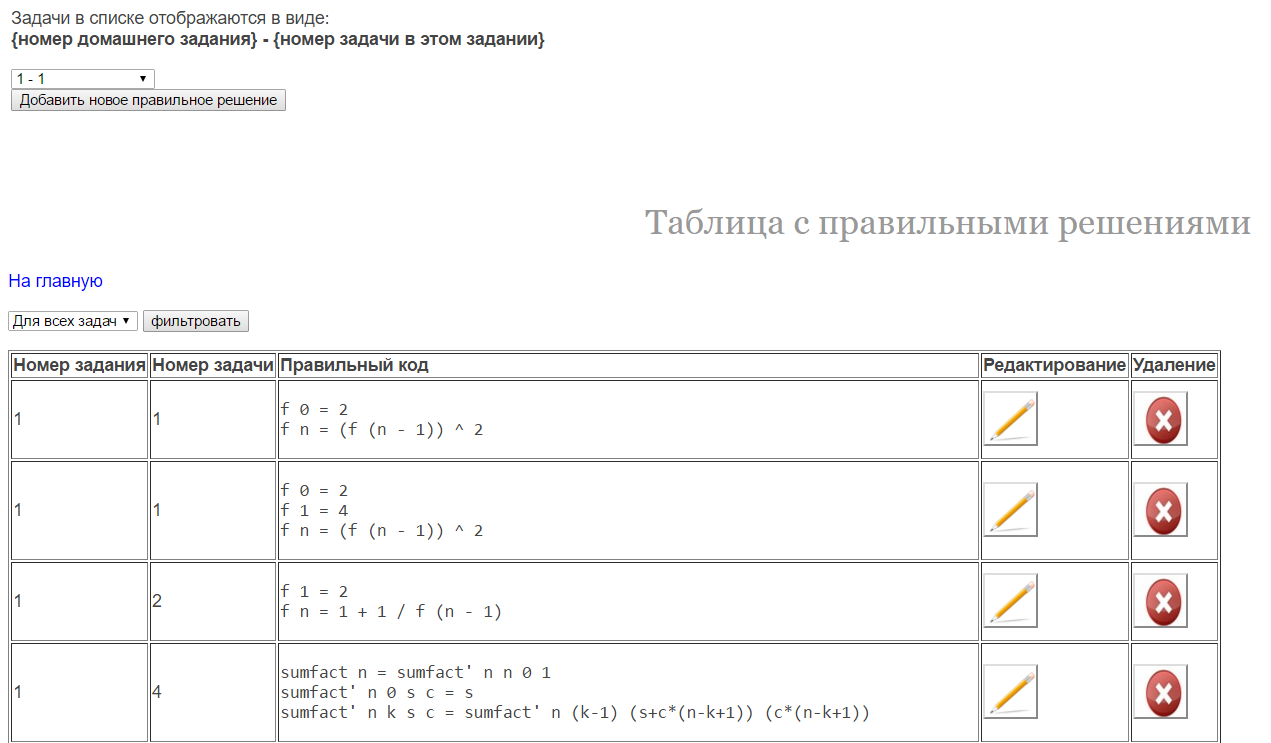
\includegraphics[width=1\linewidth]{correct.png}}
\caption{Table with the right solutions.}
\label{correct}
\end{figure}

The last two columns are responsible for editing and deleting, respectively. When editing, we get to the page where you make changes. When you delete we delete the desired right decision. At the top there is a button "Add new right decision." Clicking on it, we will get to the page to create a new right decision.

\subsection{Adding the right decisions}
Once we got to add the right solutions page (fig.~\ref{addcorrect}), we have to fill in only the very right decision, as the task number was specified on the previous page. But if you suddenly need to change it, simply enter the desired number of us in the field.
\begin{figure}[h]
\center{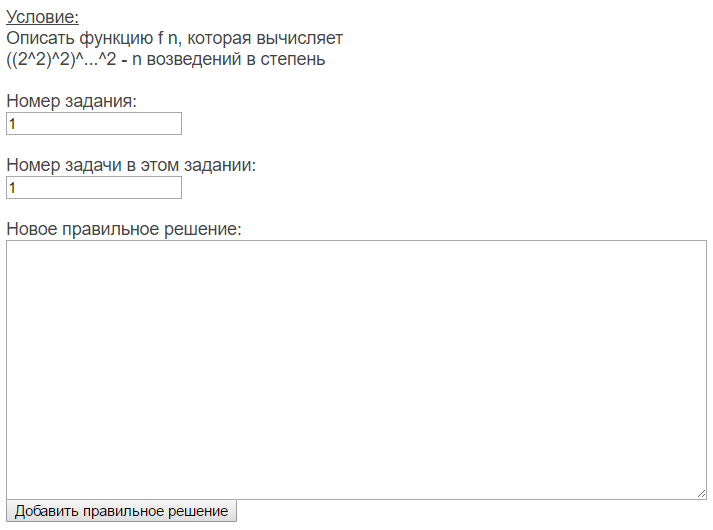
\includegraphics[width=1\linewidth]{addCorrect.png}}
\caption{Adding new right decisions.}
\label{addcorrect}
\end{figure}

\subsection{Other features}
\subsubsection*{Editing}
On the main page right decisions displays information about all the correct solution for the desired task. It is represented by vvide table, in which the penultimate column is responsible for editing the task. By clicking on the appropriate icon, we get to the edit page right decision (рис.~\ref{editcorrect}). For change task number or text solutions change the relevant data accept the changes, or they will not be saved.
\begin{figure}[h]
\center{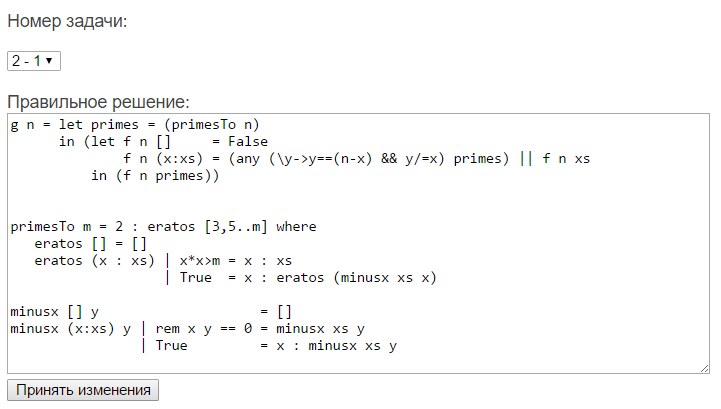
\includegraphics[width=1\linewidth]{editCorrect.png}}
\caption{Editing right decision.}
\label{editcorrect}
\end{figure}

\subsubsection*{Removal}
For each decision on the main page of correct decisions in the last column is the delete icon. When pressed, the system asks you to confirm that we want to remove this particular line. After confirmation, the corresponding row is deleted.
\subsubsection*{Selection by number problem}
Displays all the right decisions a little uncomfortable, so the teacher has the ability to filter by number problem solving. To do this, select the number of the desired task and click "Filter" button.

\subsection{The awarding of Automatic}
On the main page showing the last teacher sent students solutions (fig.~\ref{systemok}). For such solutions have a special filter, in which all the solutions that can be counted automatically labeled as "Approved system." After clicking on "solutions to credit-approved system" all such decisions will automatically be counted.
\begin{figure}[h]
\center{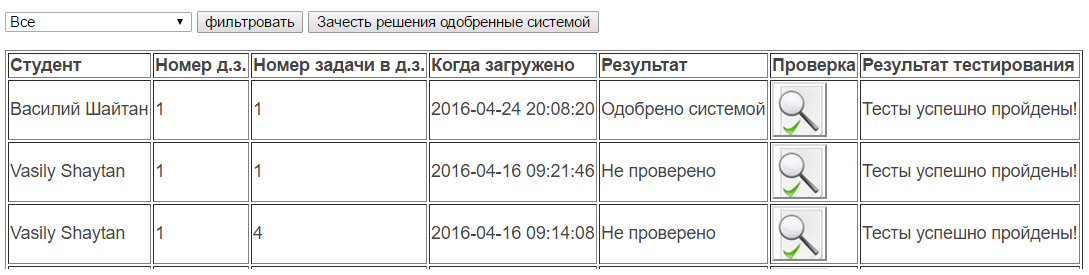
\includegraphics[width=1\linewidth]{systemOk.png}}
\caption{Decisions adopted by the system.}
\label{systemok}
\end{figure}

\subsection{List of typical comments}
On the teacher's page in the upper left corner there is a link "Typical comments". After clicking on it, we find ourselves on the page where the information is displayed on comments (рис.~\ref{remark}). Present adding, editing and deleting comments. When you press the right buttons, we get to meet these buttons page.

\begin{figure}[h]
\center{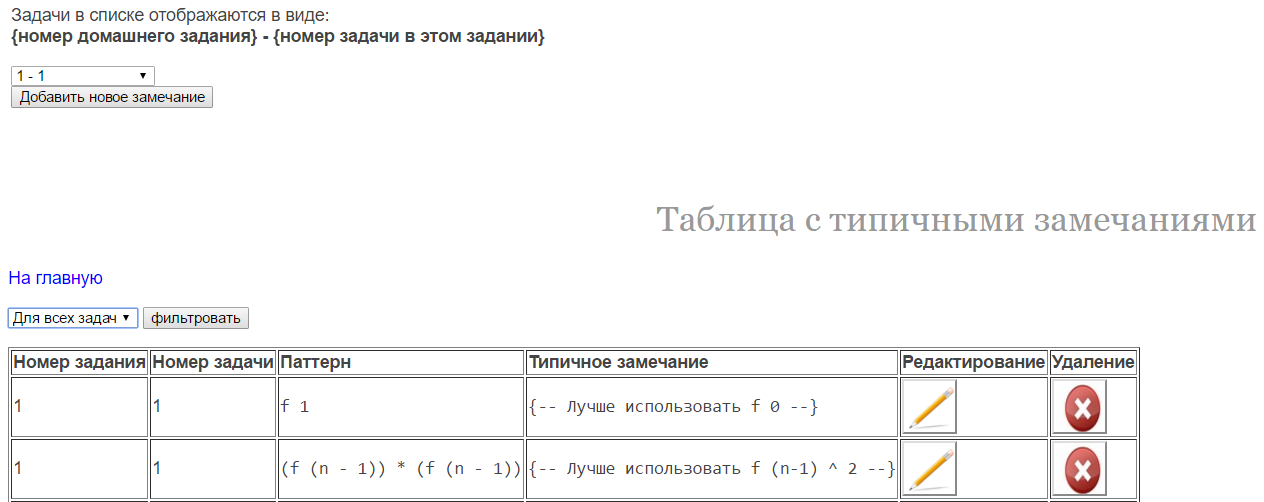
\includegraphics[width=1\linewidth]{remark.png}}
\caption{Page typical comments.}
\label{remark}
\end{figure}

\subsection{Adding a new typical comments}
Once we got to the addition of a typical page comments (рис.~\ref{addremark}), we need to fill the "new pattern" and "New typical remark." The first field we write the desired pattern, and the second, a remark which should be to bring the system when it is detected. You can change the number of tasks that point to the previous page.

\begin{figure}[h!]
\center{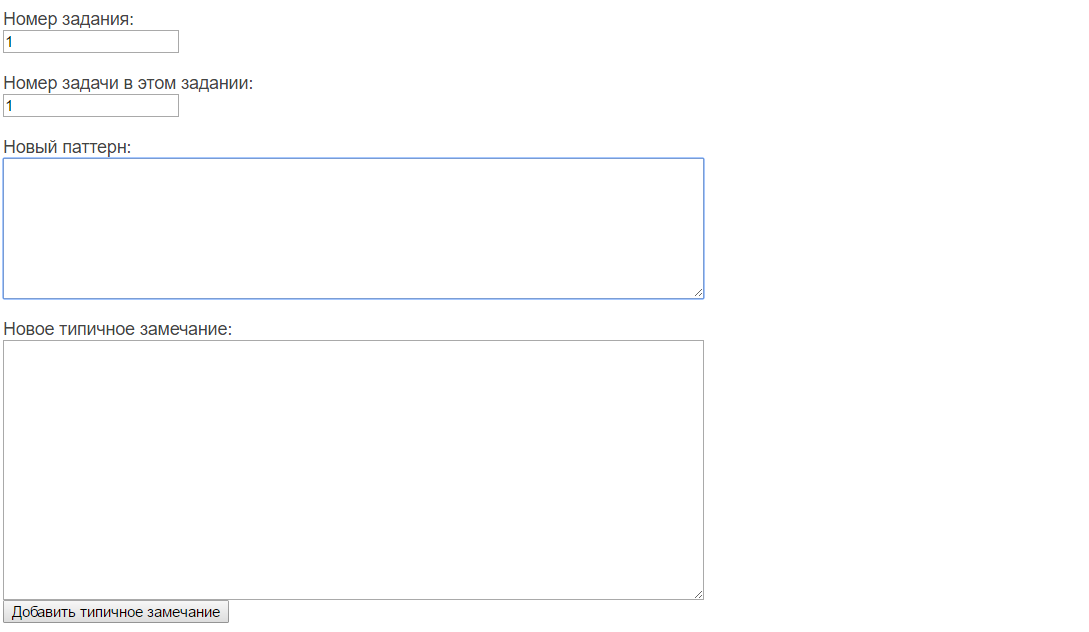
\includegraphics[width=1\linewidth]{addRemark.png}}
\caption{Adding a typical remark.}
\label{addremark}
\end{figure}

\subsection{Other features}
\subsubsection*{Editing}
On the main page of the typical comments displays information about all the observations for the required task. It is represented by vvide table, in which the penultimate column is responsible for the editing of this remark. By clicking on the appropriate icon, we get to the edit page of the typical comments. To change the sample task number or text notes, change sootvetstvyuschie data. After that, we accept the changes, or they will not be saved. An example of the typical comments edit page is shown in fig.~\ref{editremark}
\begin{figure}[h]
\center{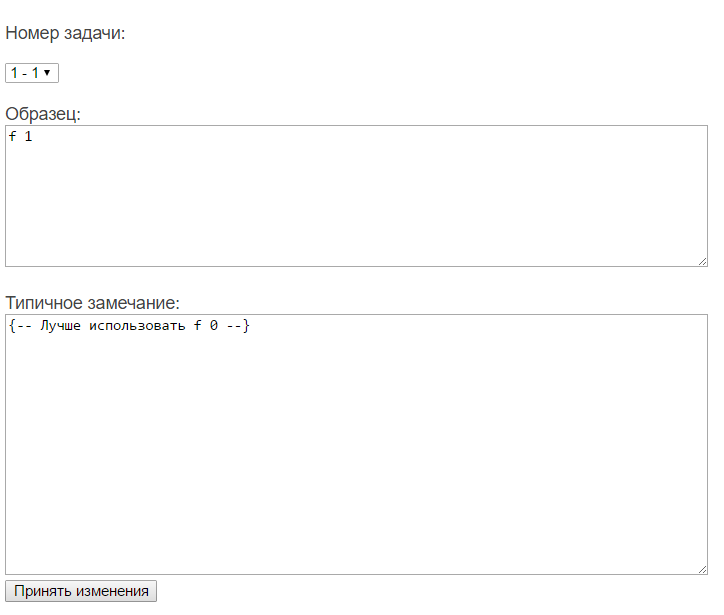
\includegraphics[width=1\linewidth]{editRemark.png}}
\caption{Editing typical comments.}
\label{editremark}
\end{figure}

\subsubsection*{Removal}
For each comment on the main page of the typical comments in the last column is the delete icon. After pressing the system asks you to confirm that we want to remove this particular row from the table. After confirmation of this line is removed.

\subsection{Verification task using typical remarks}
When checking the problems, the teacher gets to the page where he can comment on the decision, sent by the student. To do this, he has a list of comments for the task to be inserted manually, and a button that allows you to automatically insert comments (fig.~\ref{autoremark}).
\begin{figure}[h]
\center{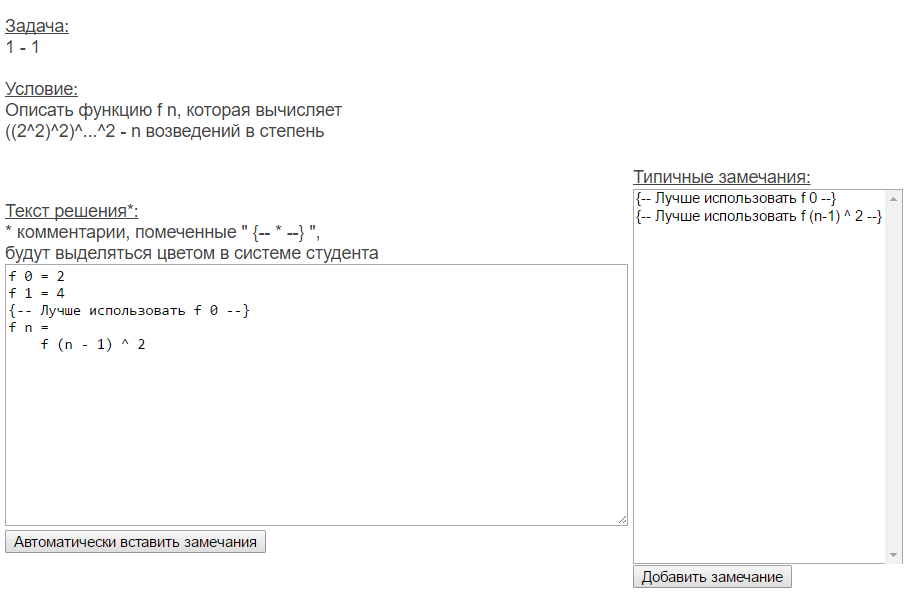
\includegraphics[width=1\linewidth]{autoRemark.png}}
\caption{The interface works with the comments.}
\label{autoremark}
\end{figure}

\subsubsection*{Manually adding typical notes}
To insert a comment in the list of comments in the student code, you need to choose a place in the code (usually the end of the line, which is the reason for the comments), where we want it
do. Next, select the desired note on the list and click "Add a comment". To save written notes, click "Save Changes." After that, the student can see his decision with the observations of the teacher, which are highlighted in red for him.

\subsubsection*{Automatic comments}
To automatically add comments to the student code, you need to check the solutions page, click the "Automatically insert a comment." Thereafter, all such comments system inserts. If you suddenly need to change the observation that the system put in, go to the field and the decision right there replacing. After not forget to save your changes.

%%%\clearpage

\section{Description of the implementation}
\label{sec:description_implementation}
%
We describe the technical improvements that have been implemented in our system.

\subsection{Driving databases}
First, it was decided to pereysti sistemamy storage MyISAM to InnoDB~\cite{innodb}. What are the reasons for the transition?
\begin{itemize}
\item InnoDB supports transactions, unlike MyISAM.
\item InnoDB supports row-level locking (MyISAM - only table-level).
\item InnoDB supports foreign key constraints (MyISAM - no).
\end{itemize}
When using transactions and foreign keys, database becomes more monolithic, disappear danger phantom records or discontinued operations. A data integrity is important wherever there is a modification of entry / update / delete. Such modifications are so many, as a new student kazhny decision is recorded in the database. Each observation of the teacher, to the left of the task requires line update in the table. \\
The database table 2 was added.
\begin{enumerate} 
\item correctsolutions - table right decisions consists of 3 fields. 
    \begin{itemize}
    \item CorrectSolutionID - primary key
    \item TaskID - task number, for which there is a right decision
    \item CorrectCode - itself the right decision
    \end{itemize}
\item tipicalremarks - Table of typical observations consists of 4 fields.
    \begin{itemize}
    \item TypicalRemarkID - primary key
    \item TaskID - task number for which there is a typical remark
    \item PatternForTaskID - sample on which we can write a remark
    \item RemarkText - text of remarks
    \end{itemize}
\end{enumerate}

\subsection{Updating outdated functions}
Since the system~\cite{ms2855.ru} was developed in 2011, the PHP programming language has undergone some changes.\\
MySQL extension date version PHP 5.5.0, and is not recommended for use when writing new code, and will be removed in the future~\cite{php.net}. It was therefore decided to use modern extension PDO (PHP Data Objects)\cite{php.net}. This extension can support any database management system, for which there is a PDO-driver. For example, PDO\_MYSQL, PDO\_IBM, PDO\_OCI, PDO\_DBLIB and many others. Since we have a MySQL database, respectively, we use the driver PDO\_MYSQL. \\
\indent All HTML tags are obsolete have been replaced by new or implemented using CSS.

\subsection{renaming variables}
Very often you can find solutions that differ only in the names of variables. For such cases, it was implemented a feature that allows you to compare the student's decision and the decision of the table right decisions. System specially renames variables. This can be seen in fig.~\ref{renamevar}. \\
All variables are replaced by x1 x2, etc.
All the same variable within a single sentence replaced with the same. Also, variables in different sentences are numbered independently, ie identical variables within a single program can have different numbers and conversely.
It is worth noting that the system performs all of these activities with the student code only after it has passed all the tests and the compilation.
\begin{figure}[h]
\center{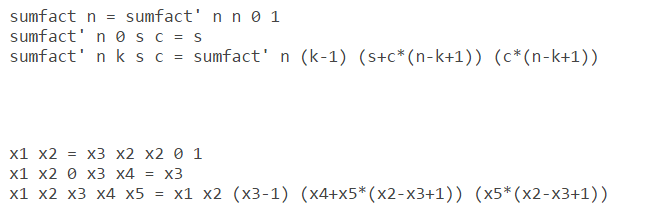
\includegraphics[width=1\linewidth]{renameVar.png}}
\caption{An example of renaming variables.}
\label{renamevar}
\end{figure}

\subsection{The structure of the project}
The project includes the n files with php, 1 file with the extension css and 1 file with the extension js. For completeness of description files is shown in Table~\ref{tr}.\\
\begin{table}[h]
\begin{center}
\begin{tabular}{|l|l|}
\hline
File & Appointment \\
\hline
authorization.php & user login page \\
config.php & Provides database connection \\
footer.php & Information Systems Authors \\
function.php & List of the basic functions \\
index.php & Home System page\\
logout.php & Implements logout \\
registration.php & User Registration Page \\ \hline
\multicolumn{2}{|c|}{Student work}\\ \hline
allDownloadSolution.php & All downloaded solutions \\
index.php & Home Student page \\
loadSolution.php & Loading solutions \\
profile.php & Page to modify personal data \\
uploadSolution.php & Output solutions \\
watchSolution.php & View solutions \\ \hline
\multicolumn{2}{|c|}{Teacher works}\\ \hline
addCorrectSolution.php & Adding the right decision \\
addTask.php & Adding a task\\
addTesk.php & Adding test\\
addTypicalRemark.php & Adding typical comments\\
checkSolution.php & Page check student solutions\\
correctSolution.php & Correct solutions \\
editCorrectSolution.php & Editing right decision \\
editTest & Editing test\\
editTypicalRemark & Editing typical comments\\
hometask.php & Hometasks \\
index.php & Home teacher page\\
result & Student results\\
task.php & Tasks \\
test.php & Tests \\
typicalRemark & Home typical comments \\ \hline
\end{tabular}
\caption{Description of the Project}
\label{tr}
\end{center}
\end{table}
%%%\clearpage

\section{Modeling the Iris Deformation}
\label{sec:patterndeformations}

Testing was conducted teacher. According to test results the following conclusions were reached:ss
\begin{itemize}
\item the awarding of a subsystem of automatic tasks works quite efficiently and facilitates verification of simple tasks.
\item expressed the wish to add to the subsystem of the automatic solution The awarding different rules of procedure
\item subsystem putting comments is also quite convenient and greatly simplifies the job of the teacher
\item it expressed the wish to allow the assignment of some observations that are applicable to all tasks
\item more complex conditions was automatically check it was desirable than that, such as the use of tail recursion, but the implementation of such checks is a rather complicated task.
\end{itemize}
The introduction of automatic subsystems The awarding decisions and automatically affixing typical observations planned for the fall semester of 2016-2017 year.


\section{Conclusion}
\label{sec:conclusion}
%
They have been developed, designed and implemented automated subsystems The awarding of tasks and automatic prostanovka comments. During testing it was demonstrated a significant labor saving teacher.

% Start of "Sample References" section

%%%\section{Typical references in new ACM Reference Format}
%%%A paginated journal article \cite{Abril07}, an enumerated
%%%journal article \cite{Cohen07}, a reference to an entire issue \cite{JCohen96},
%%%a monograph (whole book) \cite{Kosiur01}, a monograph/whole book in a series (see 2a in spec. document)
%%%\cite{Harel79}, a divisible-book such as an anthology or compilation \cite{Editor00}
%%%followed by the same example, however we only output the series if the volume number is given
%%%\cite{Editor00a} (so Editor00a's series should NOT be present since it has no vol. no.),
%%%a chapter in a divisible book \cite{Spector90}, a chapter in a divisible book
%%%in a series \cite{Douglass98}, a multi-volume work as book \cite{Knuth97},
%%%an article in a proceedings (of a conference, symposium, workshop for example)
%%%(paginated proceedings article) \cite{Andler79}, a proceedings article
%%%with all possible elements \cite{Smith10}, an example of an enumerated
%%%proceedings article \cite{VanGundy07},
%%%an informally published work \cite{Harel78}, a doctoral dissertation \cite{Clarkson85},
%%%a master's thesis: \cite{anisi03}, an online document / world wide web resource \cite{Thornburg01}, \cite{Ablamowicz07},
%%%\cite{Poker06}, a video game (Case 1) \cite{Obama08} and (Case 2) \cite{Novak03}
%%%and \cite{Lee05} and (Case 3) a patent \cite{JoeScientist001},
%%%work accepted for publication \cite{rous08}, 'YYYYb'-test for prolific author
%%%\cite{SaeediMEJ10} and \cite{SaeediJETC10}. Other cites might contain
%%%'duplicate' DOI and URLs (some SIAM articles) \cite{Kirschmer:2010:AEI:1958016.1958018}.
%%%Boris / Barbara Beeton: multi-volume works as books
%%%\cite{MR781536} and \cite{MR781537}.

%%%\appendix

%%%\section{Classical Multidimensional Scaling}
%%%\label{sec:cmds}

%%%Let $\mathrm{D}$ be an $n\times n$ matrix of pairwise distances. The
%%%matrix $D$ is symmetric with a zero diagonal. We are interested in
%%%finding a $d \times n$ matrix $\mathrm{X}$ where each column
%%%$\bm{x}_{i}$ is the representation of the point $i$ in $R^{d}$ and
%%%$\mathrm{D}_{ij} = \|\bm{x}_{i}-\bm{x}_{j}\|_{2}$. Denote the inner
%%%product (or Gram matrix) for this set of points by $\mathrm{K} =
%%%\mathrm{X}^{\top}\mathrm{X}$.


%%%$\mathrm{K}$ is an $n\times n$ symmetric positive semidefinite matrix.
%%%Let us now abuse notation and use $\mathrm{D}^{2}$ to indicate the
%%%matrix of squared pairwise distances $\mathrm{K} =
%%%-\frac{1}{2}(\mathrm{I} -
%%%\mathrm{1}\mathrm{1}^{\top})\mathrm{D}^{2}(\mathrm{I} -
%%%\mathrm{1}\mathrm{1}^{\top})$. Here, $\mathrm{I}$ is the $n \times n$
%%%identity matrix and $\mathrm{1}$ is the $n$-vector of all ones.

%%%\begin{acks}
%%%We are grateful to the following people for resources, discussions and
%%%suggestions: Prof. Jacobo Melamed Cattan (Ophthalmology-UFRGS), Prof.
%%%Roberto da Silva (UFRGS), Prof. Luis A. V. Carvalho (Optics-USP/SC),
%%%Prof. Anatolio Laschuk (UFRGS), Leandro Fernandes, Marcos
%%%Slomp, Leandro Lichtenfelz, Renato Silveira,
%%%Eduardo Gastal, and Denison Tavares. We also thank the volunteers who
%%%allowed us to collect pictures and videos of their irises: Alex Gimenes,
%%%Boris Starov, Christian Pagot, Claudio Menezes, Giovane Kuhn, Jo\~{a}o
%%%Paulo Gois, Leonardo Schmitz, Rodrigo Mendes, and Tiago Etiene.
%%%\end{acks}

% Bibliography
\bibliographystyle{ACM-Reference-Format-Journals}
\bibliography{acmtog-sample-bibfile.bib}
%% PAPEERIA-TEMPLATE\bibliography'{'{1}'}'
                                % Sample .bib file with references that match those in
                                % the 'Specifications Document (V1.5)' as well containing
                                % 'legacy' bibs and bibs with 'alternate codings'.
                                % Gerry Murray - March 2012

\received{May 2016}{June 2016}

\end{document}
% End of v2-acmtog-sample.tex (March 2012) - Gerry Murray, ACM
